\section{Kapitel 3}
\subsection{Lineare homogene Differentialgleichung 2. Ordnung}
DGL: $a \cdot y''(t) + b \cdot y'(t) + c \cdot y(t) = 0$\\
Ansatz: $y(t) = e^{\lambda t}$\\
Einsetzen in DGL $\rightarrow$ Charakteristisches Polynom: $a\lambda^2 + b\lambda +c =0$\\
Nullstellen der Gleichung bestimmen: $\lambda_1,\lambda_2 = \frac{-b \pm \sqrt{b^2 - 4ac}}{2a}$\\
Fall 1:\\ 
$\lambda_1,\lambda_2 =$ reell $\rightarrow y_1(t) = e^{\lambda_1 t}, y_2(t) = e^{\lambda_2 t}$\\
Falls 2:\\ 
$\lambda = \lambda_1 = \lambda_2 =$ reell $\rightarrow y_1(t) = e^{\lambda t}, y_2(t) = te^{\lambda t}$\\
Fall 3:\\ 
$\lambda_1,\lambda_2* =$ komplex $\rightarrow z_1(t) = e^{\lambda_1 t}, z_2(t) = e^{\lambda_2 t}$\\
$y_1(t) = Real(z_1)$ und $y_2(t) = Imag(z_1)$\\
Allgemeine Lösung: $y(t) = c_1y_1(t) + c_2y_2(t)$\\
Freiheitsgrade $c_1,c_2$ mit Hilfe der gegebenen Anfangsbedinungen bestimmen. 
\subsection{Umwandlung in ein System 1. Ordnung}
$a \cdot y''(t) + b \cdot y'(t) + c \cdot y(t) = 0$\\
Substitution:\\
$x_1(t) = y(t)$\\
$x_2(t) = y'(t)$\\
$
	\begin{vmatrix} 
	        y'(t)\\ 
	        y''(t)\\   
	\end{vmatrix}
	=
	\begin{vmatrix} 
	        x_1'(t)\\ 
	        x_2'(t)\\   
	\end{vmatrix}
	=
	\begin{vmatrix} 
	        x_2(t)\\ 
	        -\frac{b}{a} - \frac{c}{a}x_1(t)\\   
	\end{vmatrix}
$\\
DGL System:\\
\begin{equation*}
x'(t) = Ax(t)
\end{equation*}
\begin{equation*}
	\begin{vmatrix} 
	        x_1'(t)\\ 
	        x_2'(t)\\   
	\end{vmatrix}
	=
	\begin{vmatrix} 
	        0 && 1\\ 
	       -\frac{c}{a} && -\frac{b}{a}\\   
	\end{vmatrix}
	\begin{vmatrix} 
	        x_1(x)\\ 
	        x_2(x)\\   
	\end{vmatrix}
\end{equation*}

Das DGL System kann nun wie ein homogenes, autonomes DGL System 1. Ordnung gelöst werden. Die Lösung für $x_1(t)$ ist geraade die Lösung der DGL 2. Ordnung, weil $x_1(t) = y(t)$, die Lösung $x_2(t)$ kann als Zwischenresultat betrachtet werden. 
Hat das DGL System 2.Ordnung noch eine Störung $g(t)$, so sieht das äquivalente System 1. Ordnung wie folgt aus:\\
\begin{equation*}
x'(t) = Ax(t) + g(t)
\end{equation*}
\begin{equation*}
	\begin{vmatrix} 
	        x_1'(t)\\ 
	        x_2'(t)\\   
	\end{vmatrix}
	=
	\begin{vmatrix} 
	        0 && 1\\ 
	       -\frac{c}{a} && -\frac{b}{a}\\   
	\end{vmatrix}
	\begin{vmatrix} 
	        x_1(t)\\ 
	        x_2(t)\\   
	\end{vmatrix}
	+
	\begin{vmatrix} 
	        0\\ 
	        g(t)\\   
	\end{vmatrix}
\end{equation*}
\subsection{Inhomogen 2. Ordnung}
\begin{tabbing}
1. Homogenes System lösen \= $a \cdot y''(t) + b \cdot y'(t) + c \cdot y(t) = 0$\\
2. Inhomogener Ansatz \> $a \cdot y''(t) + b \cdot y'(t) + c \cdot y(t) = g(t)$\\
\>\begin{tabular}{|l|l|}
	\hline
	\textbf{Inhomogenität}              & \textbf{Ansatz} \\ \hline
	$g(t)=a_0\,t^n + ... + a_n$        & $y(t) = t^s(A_0\,t^n + ... + A_n)$ \\ \hline
	$g(t)=(a_0\,t^n + ... + a_n)e^{\alpha \, t}$  & $y(t) = t^s(A_0\,t^n + ... + A_n)e^{\alpha \, t}$ \\ \hline
	$g(t)=(a_0\,t^n + ... + a_n)e^{\alpha \, t}sin(\beta \, t)$
		& $y(t) = t^s(A_0\,t^n + ... + A_n)e^{\alpha \, t}sin(\beta \, t) + $ \\ 
	oder $(a_0\,t^n + ... + a_n)e^{\alpha \, t}cos(\beta \, t)$ 
		&$t^s(B_0\,t^n + ... + B_n)e^{\alpha \, t}cos(\beta \, t)$ \\ \hline
\end{tabular}\\
\> $s = [0,1,2]$, so dass kein Summand Lösung der homogenen Gleichung.\\
3. Zusammensetzen \> $y(t)=y_h(t)+y_p(t)$
\end{tabbing}
\subsection{Variation der Konstanten}
Hat man eine lineare, inhomogene Differentialgleichung 2. Ordnung mit folgender Struktur:\\
\begin{equation*}
y''(t) + p(t)y'(t) + q(t)y(t) = g(t)
\end{equation*}

Um die Variation der Konstanten verwenden zu  können, muss das System in ein System 1. Ordnung gebracht werden:\\
\begin{equation*}
x'(t) = A(t)x(t) + b(t)
\end{equation*}
\begin{equation*}
	\begin{vmatrix} 
	        y'(t)\\ 
	        y''(t)\\   
	\end{vmatrix}
	=
	\begin{vmatrix} 
	        x_1'(t)\\ 
	        x_2'(t)\\   
	\end{vmatrix}
	=
	\begin{vmatrix} 
	        0 && 1\\ 
	       -q(t) && -p(t)\\   
	\end{vmatrix}
	\begin{vmatrix} 
	        x_1(t)\\ 
	        x_2(t)\\   
	\end{vmatrix}
	+
	\begin{vmatrix} 
	        0\\ 
	        g(t)\\   
	\end{vmatrix}
\end{equation*}
In einem ersten Schritt wird die homogene Gleichung gelöst und wir erhalten zwei Fundementallösungen $y_1(t)$ und $y_2(t)$, damit erhalten wir eine Fundamentalmatrix der Form: \\
\begin{equation*}
X(t) = 
	\begin{vmatrix} 
	        y_1(t) && y_2(t)\\ 
	        y_1'(t) && y_2'(t)\\ 
	\end{vmatrix}
\end{equation*}
Um nun die partikuläre Lösung zu erhalten, verwenden wir folgende Gleichung: 
\begin{equation*}
y_P(t) = X(t) \int{X(t)^{-1}b(t)dt}
\end{equation*}
Die gesamte Lösung ergibt sich dann wieder aus der Summe der homogenen sowie der partikulären Lösung. 
\subsection{Schwingungen}

\begin{tabular}{|l|l|}
	\hline
	\textbf{Terminologie}              & \textbf{Gleichung} \\ \hline
	freie ungedämpfte Schwingung       & $m \cdot y''(t) + k \cdot y(t) = 0$ \\ \hline
	freie gedämpfte Schwingung         & $m \cdot y''(t) + \gamma\cdot y'(t) + k \cdot y(t) = 0$ \\ \hline
	erzwungene ungedämpfte Schwingung  & $m \cdot y''(t) + k \cdot y(t) = F(t)$ \\ \hline
	erzwungene gedämpfte Schwingung    & $m \cdot y''(t) + \gamma\cdot y'(t) + k \cdot y(t) = F(t)$ \\ \hline
\end{tabular}\\

\textbf{Matrixschreibweise}\\
$ y''(t) + p(t)\cdot y'(t) + q(t) \cdot y(t) = g(t) \rightarrow x' = A \cdot x + b \quad 
A(t)=\begin{bmatrix}
 0 & 1 \\
 -q(t) & -p(t)\\
\end{bmatrix} \quad
b(t)=\begin{bmatrix}
 0 \\
 g(t)\\
\end{bmatrix}$

\subsubsection{Freie Schwingung}
$m \cdot y''(t) + \gamma\cdot y'(t) + k \cdot y(t) = 0$\\
\begin{tabbing}
ohne Dämpfung ($\gamma = 0$): \= $y(t) = A \cdot cos(w_0 \cdot t) + b\cdot sin(w_0 \cdot t) \quad w_0=\sqrt{\dfrac{k}{m}} \quad  A=y_0 \quad B=\dfrac{y_0'}{w_0}$\\
\>$y(t) =R\cdot cos(w_0 \cdot t - \varphi) \quad R=\sqrt{A^2+B^2} \quad \varphi=atan2(B,A)$\\
\end{tabbing}

\begin{tabbing}
mit Dämpfung ($\gamma \neq 0$): \= $Z(\lambda)=m\lambda^2 + \gamma \lambda + k \rightarrow \lambda_{1,2}=\dfrac{-\gamma \pm \sqrt{\gamma^2 - 4 \, m \, k}}{2 \, m} \rightarrow D=\gamma^2 - 4 \, m \, k$\\
\> Fall 1: $D>0 \quad y(t)=Ae^{\lambda_1 \, t} + Be^{\lambda_2 \, t}$\\
\> Fall 2: $D=0 \quad y(t)=(A + B \,t)e^{\lambda \, t}$\\
\> Fall 3: $D<0 \quad y(t)=Ae^{\mu \, t}cos(\nu \, t) + Be^{\mu \, t}sin(\nu \, t) \quad \mu=-\dfrac{\gamma}{2\,m} \quad \nu = \sqrt{\dfrac{k}{m}-\dfrac{\gamma^2}{4 \, m^2}}$
\end{tabbing}

$\operatorname{atan2}(B, A) = \begin{cases}
\arctan\left(\frac B A\right) & \qquad A > 0 \\
\arctan\left(\frac B A\right) + \pi& \qquad B \ge 0 , A < 0 \\
\arctan\left(\frac B A\right) + 2\pi& \qquad B < 0 , A < 0 \\
+\dfrac{\pi}{2} & \qquad B > 0 , A = 0 \\
+\dfrac{3\pi}{2} & \qquad B < 0 , A = 0 \\
\text{undefined} & \qquad B = 0, A = 0
\end{cases}$

\subsubsection{Erzwungene Schwingung}
$m \cdot y''(t) + \gamma\cdot y'(t) + k \cdot y(t) = f(t)=Ae^{i\,w\,t} \rightarrow$\\
$ y''(t) + 2 \, \delta y'(t) + w_0^2 \, y(t) = F(t)$ mit $w_0=\sqrt{\dfrac{k}{m}} \quad \delta=\dfrac{\gamma}{2\,m} \quad F(t)=\dfrac{f(t)}{m}$\\
$\rightarrow y(t)=y_h(t)+y_p(t)$

\begin{tabbing}
ohne Dämpfung ($\delta = 0$): \= $y(t) = \dfrac{A}{w_0^2-w^2}(cos(w_0\,t)-cos(w\,t))$\\
\> $y(t) = \dfrac{A}{w_0^2-w^2}sin(\dfrac{w_0-w}{2} \cdot t)sin(\dfrac{w_0+w}{2} \cdot t)$\\
\end{tabbing}

\begin{tabbing}
mit Dämpfung ($\delta \neq 0$): \= $y_h(t \rightarrow \infty) = 0$\\
\> $y_p(t)= \dfrac{1}{w_0^2-w^2 + 2\,i\,\delta\,w}Ae^{i\,w\,t}$\\
\> $y_p(t)= g(w)\,A\,cos(wt-\varphi(w))$\\
\> $g(w)=\dfrac{1}{\sqrt{(w_0^2-w^2)^2+4\delta^2w^2}} \quad \varphi(w)=arccos(\dfrac{w_0^2-w^2}{\sqrt{(w_0^2-w^2)^2+4\delta^2w^2}})$\\
\> $g_{max}=\dfrac{1}{2\delta} \dfrac{1}{\sqrt{w_0^2-\delta^2}}$ bei $w_{max}=\sqrt{w_0^2-2\,\delta^2}$
\end{tabbing}
\begin{minipage}[h]{0.5\textwidth} 
	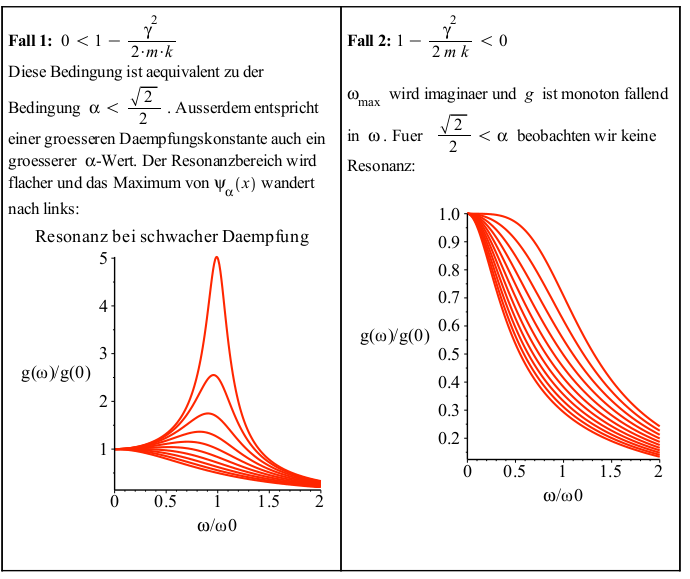
\includegraphics[width=1.0\textwidth]{images/Erzwungen1.png}
\end{minipage}
\begin{minipage}[h]{0.5\textwidth}
	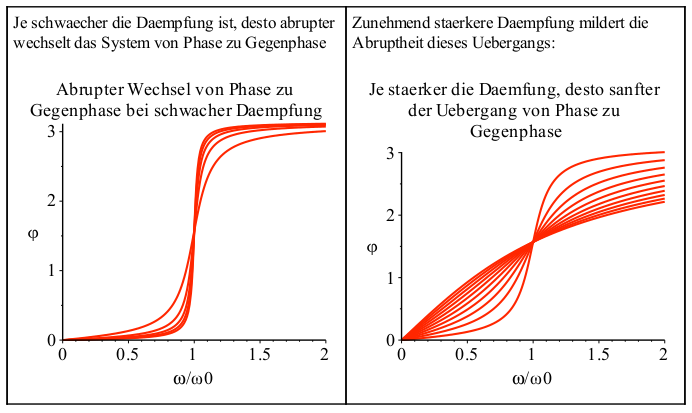
\includegraphics[width=1.0\textwidth]{images/Erzwungen2.png}
\end{minipage}